\subsection{模拟题参考答案}
1. 偏微方程只给出初始条件时称为\textbf{初值}问题.

2. 解的\textbf{存在、唯一性和稳定性}称为问题的适定性.

3. 三维 Laplace 方程的基本解是
$
v=-\dfrac{1}{4 \pi r}=-\dfrac{1}{4 \pi \sqrt{\left(x-x_{0}\right)^{2}+\left(y-y_{0}\right)^{2}+\left(z-z_{0}\right)^{2}}}.
$

4. 二维齐次热传导方程的一般形式为$ u_t = a^2(u_{xx} +u_{yy})$.

5. $ u_{t}-\left(u_{x x}+u_{y y}\right)=0 $ 是\textbf{抛物型}偏微分方程.

6. 说明物理现象初始状态的条件叫\textbf{初始条件} , 说明边界约束情况的条件叫\textbf{边界条件}.

7.边界条件 $ \left.\left(\frac{\partial u}{\partial n}+\sigma u\right)\right|_{\partial \Omega}=f $ 是\textbf{第三类}边界条件, 其中 $ \partial \Omega $ 为边界.

\begin{questions}

\question{
下列不是调和函数的是 ( )

A. $ u(x, y)=e^{x} \sin y $

B. $ u(x, y)=x^{2}+y^{2} $

C. $ u(x, y)=a x+b y+c $

D. $ u(x, y)=x^{3}-3 x y^{2} $
}
\begin{solution}
   我们可以使用拉普拉斯算子 $\Delta u$ 来验证哪个函数是调和函数。调和函数满足 $\Delta u = 0$。让我们使用 $\Delta u$ 来验证每个选项:

A. $u(x, y) = e^x \sin y$:
$$\Delta u = \frac{\partial^2 u}{\partial x^2} + \frac{\partial^2 u}{\partial y^2} = e^x \sin y - e^x \sin y = 0$$

由于 $\Delta u$ 等于零,所以 A 是调和函数。

B. $u(x, y) = x^2 + y^2$:
$$\Delta u = \frac{\partial^2 u}{\partial x^2} + \frac{\partial^2 u}{\partial y^2} = 2 + 2 = 4$$

由于 $\Delta u$ 不等于零,所以 B 不是调和函数。

C. $u(x, y) = ax + by + c$:
$$\Delta u = \frac{\partial^2 u}{\partial x^2} + \frac{\partial^2 u}{\partial y^2} = 0$$

由于 $\Delta u$ 等于零,所以 C 是调和函数。

D. $u(x, y) = x^3 - 3xy^2$:
$$\Delta u = \frac{\partial^2 u}{\partial x^2} + \frac{\partial^2 u}{\partial y^2} = 6x - 6x = 0$$

由于 $\Delta u$ 等于零,所以 D 也是调和函数。

因此A, C ,D 都是调和函数,只有 B 不是调和函数。
\end{solution}
\question{
设 $ G\left(M, M_{0}\right) $ 为区域 $ \Omega $ 上 Laplace 方程 $ \Delta u=0 $ Dirichlet 问题的 Green 函数,
则 $$ \iint_{\partial \Omega} \frac{\partial G\left(M, M_{0}\right)}{\partial \vec{\boldsymbol n}} d S_{M}=(\quad) $$

$$\mathrm{A}. 0\quad\quad\quad\quad \mathrm{B}. 1\quad\quad\quad\quad \mathrm{C}. -1\quad\quad\quad\quad \mathrm{D}.\text{不确定}$$

}
\begin{solution}
   狄利克雷问题 
$$\left\{\begin{array}{l}\Delta u=0,(x, y, z) \in \Omega \\ \left.u\right|_{\partial \Omega}=\varphi(M), M \in \partial \Omega\end{array}\right. $$
的解可表示为 
$$ u\left(M_{0}\right)=-\iint_{\partial \Omega} \varphi(M) \cdot \frac{\partial G\left(M, M_{0}\right)}{\partial n} d S_{M} $$
显然 $ u \equiv 1 $ 是如下边值问题
$$
\begin{array}{l}
\left\{\begin{array}{l}
\Delta u=0 \quad M \in \Omega\\
\left.u\right|_{\partial \Omega}=1
\end{array} \right.
\end{array} 
$$
的解.为此取$\varphi(M)=1$即得
$$
\iint_{\partial \Omega} \frac{\partial G\left(M, M_{0}\right)}{\partial n} d S_{M}=-1
$$
\end{solution}
\question{
考虑常微分方程特征值问题
$$
\begin{array}{l}
\dfrac{d^{2} X(x)}{d x^{2}}+\lambda X(x)=0,0<x<\pi, \\
X(0)=0, X(\pi)=0,
\end{array}
$$
不是该问题的特征值的是 ( )
$$\mathrm{A}. 1\quad\quad\quad\quad \mathrm{B}. 3\quad\quad\quad\quad \mathrm{C}. 4\quad\quad\quad\quad \mathrm{D}.16$$
}
\begin{solution}
求解特征值和特征函数的问题:
$$
\left\{\begin{array}{l}
X^{\prime \prime}+\lambda X=0 \\
X(0)=0, X(\pi)=0
\end{array} .\right.
$$
为了求解这个特征值问题, 需要分下面三种情形讨论:

1. 当 $ \lambda<0 $ 时, 方程 $ X^{\prime \prime}+\lambda X=0 $ 的通解为
$$
X(x)=A \mathrm{e}^{\sqrt{-\lambda} x}+B \mathrm{e}^{-\sqrt{-\lambda} x}
$$
其中, $ A, B $ 为两个任意常数. 代入边界条件, 得
$$
X(0)=A \cdot 1+B \cdot 1=0, \quad X(\pi)=A \mathrm{e}^{\sqrt{-\lambda} \pi}+B \mathrm{e}^{-\sqrt{-\lambda} \pi}=0
$$
因为
$$
\left|\begin{array}{cc}
1 & 1 \\
\mathrm{e}^{\sqrt{-\lambda }\pi}& \mathrm{e}^{-\sqrt{-\lambda } \pi}
\end{array}\right| \neq 0,
$$
故 $ A=B=0 $, 即有 $ X(x) \equiv 0 $.
所以, 当 $ \lambda<0 $ 时, 方程 $ X^{\prime \prime}+\lambda X=0 $ 的边值问题只有零解.

2. 当 $ \lambda=0 $ 时, 方程 $ X^{\prime \prime}+\lambda X=0 $ 的通解为 $ X=A x+B $. 其中 $ A, B $ 为两个任意常数. 代入边界条件, 得
$$
X(0)=A \cdot 0+B=0, X(\pi)=A \cdot \pi+B=0 .
$$
从而 $ A=B=0 $. 此时, 方程 $ X^{\prime \prime}+\lambda X=0 $ 的边值问题也只有零解.

3. 当 $ \lambda>0 $ 时, 方程 $ X^{\prime \prime}+\lambda X=0 $ 的通解为
$$
X(x)=A \cos \sqrt{\lambda} x+B \sin \sqrt{\lambda} x .
$$
代入边界条件, 得
$$
X(0)=A \cdot 1+B \cdot 0=0, \quad X(L)=A \cos \sqrt{\lambda} \pi+B \sin \sqrt{\lambda} \pi=0 .
$$
即 $ A=0, B \sin \sqrt{\lambda} \pi=0 $. 为了使 $ X(x) $ 不恒为零, 应有 $ B \neq 0 $, 即 $ \sin \sqrt{\lambda} \pi=0 $. 于是, 得 $ \sqrt{\lambda} \pi=k \pi, k=1,2, \cdots $. 满足这等式的 $ \lambda $ 值就是特征值, 记为 $ \lambda_{k}: $
$$
\lambda_{k}=k^{2} , k=1,2, \cdots
$$
因此$\lambda$可以取1,4,9,而不可能为3.
\end{solution}
\question{
设 $ u $ 是单位圆盘 $ \Omega $ 上的调和函数, 则其在 $ \overline{\Omega} $ 上的最大值不可能在点( )达到
$$ \mathrm{A.}(0,0) \quad\quad\quad\quad \mathrm{B.}(0,1)  \quad\quad\quad\quad\mathrm{C.}(1,0)\quad\quad\quad\quad  \mathrm{D.}(-1,0) $$
}
\begin{solution}
    $ \mathbb{R}^{n} $ 中一个有界区域 $ \Omega $ 上的调和函数一定在边界 $ \partial \Omega $ 上达到 $ \overline{\Omega} $ 上的最大值和最小值, 即
$$
\max _{x \in \overline{\Omega}} u=\max _{x \in \partial \Omega} u, \quad \min _{x \in \overline{\Omega}} u=\min _{x \in \partial \Omega} u .
$$

根据调和函数的上述性质,如果 $u$ 是单位圆盘 $\Omega$ 上的调和函数,则 $u$ 在 $\overline{\Omega}$上的最大值只能出现在 $\partial \Omega$ 上。因此在平面的圆周上的任意一点均有可能取最大值,而在圆内的点(0,0)上不可能取到最大值.

因此,在选项中,最大值不可能出现在点 $(0,0)$ (选项 A)
\end{solution}

\question{
一维波动方程初值问题
$$
\left\{\begin{array}{ll}
u_{t t}-u_{x x}=0,&-\infty<x<\infty, \\
u(x, 0)=\sin x, u_{t}(x, 0)=0,&-\infty<x<\infty,
\end{array}\right.
$$
解为 ( )

$$ \begin{array}{llll}\mathrm{A.} \sin x \cos t & \mathrm{~B.} \sin x \sin t & \mathrm{C.} \frac{\sin x \cos t}{2} & \mathrm{D.} 2 \sin x \sin t\end{array} $$
}
\begin{solution}
    根据达朗贝尔公式
$$
u(x, t)=\frac{1}{2}[\varphi(x+a t)+\varphi(x-a t)]+\frac{1}{2 a} \int_{x-a t}^{x+a t} \psi(\xi) d \xi
$$
由题意 $ a=1 . \quad \varphi(x)=\sin x , \psi(x)=0$.
即
$$u(x, t)=\frac{1}{2}[\sin (x+t)+\sin (x-t)]=\sin x\cdot\cos t \text { (积化和差公式) }$$
\end{solution}
\end{questions}

\begin{questions}
\question{
 求解齐次波动方程初值问题
$$
\left\{\begin{array}{l}
u_{t t}-a^{2} u_{x x}=0,-\infty<x<\infty, \\
u(x, 0)=\sin x, u_{t}(x, 0)=\cos x,-\infty<x<\infty .
\end{array}\right.
$$
}
\begin{solution}
直接利用达朗贝尔公式
$$
\begin{aligned}
u(x, t) & =\frac{1}{2}[\sin (x+a t)+\sin (x-a t)]+\frac{1}{2 a} \int_{x-a t}^{x+a t} \cos \xi d \xi \\
& =\sin x \cdot \cos a t+\left.\frac{1}{2 a} \sin \xi\right|_{x-a t} ^{x+a t} \\
& =\sin x \cdot \cos a t+\frac{1}{2 a}[\sin (x+a t)-\sin (x-a t)] \\
& =\sin x \cdot \cos a t+\frac{1}{a} \cos x \sin a t
\end{aligned}
$$
\end{solution}
\question{ 求解非齐次波动方程的初值问题
$$
\begin{array}{l}
u_{t t}-a^{2} u_{x x}=2 x t,-\infty<x<\infty, t>0, \\
u(x, 0)=x^{2}, u_{t}(x, 0)=\sin 2 x .
\end{array}
$$}
\begin{solution}
    直接利用一维非齐次波动方程的初值问题的解表达式,有
$$
\begin{aligned}
& u(x, t)=\frac{1}{2}[\varphi(x+a t)+\varphi(x-a t)]+\frac{1}{2 a} \int_{x-a t}^{x+a t} \psi(\xi) d \xi \\
+ & \frac{1}{2 a} \int_{0}^{t} \int_{x-a(t-\tau)}^{x+a(t-\tau)} f(\xi, \tau) d \xi d \tau \\
= & \frac{1}{2}\left[(x+a t)^{2}+(x-a t)^{2}\right]+\frac{1}{2 a} \int_{x-a t}^{x+a t} \sin 2 \xi d \xi \\
+ & \frac{1}{2 a} \int_{0}^{t} \int_{x-a(t-\tau)}^{x+a(t-\tau)} 2 \xi \tau d \xi d \tau \\
= & x^{2}+a^{2} t^{2}+\frac{1}{2 a} \sin 2 x \sin 2 a t+\frac{1}{3} x t^{3}
\end{aligned}
$$

\hrule

具体分析:

上述问题中的方程和定解条件都是线性的所以根据叠加原理,将上述定解问题分解为以下两个定解问题:

$$(1) \left\{\begin{array}{l}u_{t t}-a^{2} u_{x x}=0 \\ u(x, 0)=x^{2}, u_{t}(x, 0)=\sin 2 x\end{array}\right. $$
$$(2) \left\{\begin{array}{l}u_{t t}-a^{2} u_{x x}=2 x t \\ u(x, 0)=0, u_{t}(x, 0)=0\end{array}\right. $$
令$u=u_{1}(x, t)+u_{2}(x, t)$

对于问题(1),我们利用达朗贝公式求解
$$
\begin{aligned}
u(x, t) & =\frac{1}{2}[u(x+a t)+v(x-a t)]+\frac{1}{2 a} \int_{x-a t}^{x+a t} \psi(\xi) d \xi \\
& =\frac{1}{2}\left[(x+a t)^{2}+(x-a t)^{2}\right]+\frac{1}{2 a} \int_{x-a t}^{x+a t} \sin 2 \xi d \xi \\
& =x^{2}+a^{2} t^{2}+\left.\frac{1}{2 a}\left(-\frac{1}{2} \cos 2 \xi\right)\right|_{x-a t} ^{x+a t} \\
& =x^{2}+a^{2} t^{2}-\frac{1}{4 a}[\cos (2 x+2 a t)-\cos (2 x-2 a t)] \\
& =x^{2}+a^{2} t^{2}+\frac{1}{2 a} \sin 2 x \cdot \sin 2 a t \quad \text { (积化和差公式) }
\end{aligned}
$$

对于问题 (2)我们利用齐次化原理求解, 由齐次化原理
$$
 u_{2}(x, t)=\int_{0}^{t} w(x, t, \tau) d \tau
$$
其中 $ w(x, t, \tau) $ 是  
$$ (3) \left\{\begin{array}{l}w_{t t}=a^{2} \omega_{x x}, t>\tau \\ \left.w\right|_{t=\tau}=0 \\ \left.w_{t}\right|_{t=\tau}=f(x, \tau)=2 x \tau\end{array}\right. $$
的解

令 $ y=t-\tau $, 则定解问题(3) 化为
$$
\left\{\begin{array}{l}
w_{t t}=a^{2} w_{y y} \\
w_{y=0}=0 \leftarrow \text { 对应 } \varphi(x) \\
\left.w_{t}\right|_{y=0}=2 x \tau \leftarrow \text { 对应 } \psi(x)
\end{array}\right.
$$
由达朗贝尔公式
$$
\begin{aligned}
w(x, t, \tau) & =\frac{1}{2}[\varphi(x+a t)+\varphi(x-a t)]+\frac{1}{2 a} \int_{x-a y}^{x+a y} f(\xi, \tau) d \xi \\
& =\frac{1}{2 a} \int_{x-a \mid t-\tau)}^{x+a(t-\tau)} 2 \xi \tau d \xi
\end{aligned}
$$
则 
$$
\begin{aligned}
 u_{2}(x, t)&=\frac{1}{2 a} \int_{0}^{t} \int_{x-a(t-\tau)}^{x+a(t-\tau)} 2 \xi \tau d \xi d \tau \\
&=\left.\frac{1}{2 a} \int_{0}^{t} \tau \cdot \xi^{2}\right|_{x-a(t-\tau)} ^{x+a(t-\tau)} d \tau \\
&=\frac{1}{2 a} \int_{0}^{t} 4 a x(t-\tau) \cdot \tau d \tau \\
&=2x \int_{0}^{t}\left(t \tau-\tau^{2}\right) d \tau \\
&=2\left.x\left(\frac{1}{2} t \tau^{2}-\frac{1}{3} \tau^{3}\right)\right|_{0} ^{t} \\
&=2x\left(\frac{1}{2} t^{3}-\frac{1}{3} t^{3}\right)=\frac{1}{3} x t^{3}
\end{aligned}
$$
因此 $ u(x, t)=u_{1}(x, t)+u_{2}(x, t) $
$$
\begin{aligned}
u(x,t) & =u_{1}(x, t)+u_{2}(x, t) \\
& =x^{2}+a^{2} t^{2}+\frac{1}{3} x t^{3}+\frac{1}{2 a} \sin 2 x \sin 2 a t
\end{aligned}
$$

\end{solution}
\question{
用分离变量法求解如下热传导方程初边值问题
$$
\left\{\begin{array}{l}
u_{t}-a^{2} u_{x x}=0,0<x<l, t>0, \\
u(0, t)=u(l, t)=0, \\
u(x, 0)=\cos x .
\end{array}\right.
$$
}
\begin{solution}
    先求满足方程和边条件的分离变量形如:
$$
u(x, t)=X(x) \cdot T(t)
$$
的非零解. 其中 $ X(x), T(t) $ 为待定函数.
把$u(x,t)$代入方程 $u_{t}-a^{2} u_{x x}=0$  得
$$
X(x) T^{\prime}(t)=a^{2} X^{\prime \prime}(x) T(t),
$$
即 
$$\frac{T^{\prime}(t)}{a^{2} T(t)}=\frac{X^{\prime \prime}(x)}{X(x)}=-\lambda $$

由于上式左端与 $ x $ 无关,而右端与 $ t $ 无关, 故它为常数. 用 $ -\lambda $表示它, 于是得两个常微分方程:
$$
\begin{array}{c}
T^{\prime}(t)+a^{2} \lambda T(t)=0, \\
X^{\prime \prime}(x)+\lambda X(x)=0
\end{array}
$$
通过解两个常微分方程来决定 $ T(t), X(x) $.  代入初始条件得:
$$
\begin{array}{l}
u(0, t)=X(0) T(t)=0 \\
u(l, t)=X(l) T(t)=0 .
\end{array}
$$
因为求非零解, 故 $ T(t) \neq 0 $, 因此得
$$
X(0)=X(l)=0
$$
(i) 先求如下问题的解:
$$
\left\{\begin{array}{l}
X^{\prime \prime}(x)+\lambda X(x)=0, \\
X(0)=X(l)=0 .
\end{array}\right.
$$
方程$X^{\prime \prime}(x)+\lambda X(x)=0$的通解依赖 $ \lambda $ 的取不同值而不同, 下面分三种情况讨论 $ \lambda $.

当 $ \lambda \leqslant 0 $ 时, 无非零解 .

当 $ \lambda>0 $ 时, 通解为
$$
X(x)=C_{1} \cos \sqrt{\lambda} x+C_{2} \sin \sqrt{\lambda} x
$$
同时又满足初始条件时, 则得:
$$
\begin{array}{c}
X(0)=C_{1}=0, \\
X(l)=C_{2} \sin \sqrt{\lambda} l=0, \text { 即 } C_{2} \sin \sqrt{\lambda} l=0 .
\end{array}
$$

当 $ C_{2} \neq 0 $ 时, 则 $ \sin \sqrt{\lambda} l=0 $,
$$
\sqrt{\lambda} l=k \pi,
$$
特征值为:
$$
\lambda_{k}=\left(\frac{k \pi}{l}\right)^{2} \quad k=1,2 \cdots,
$$
其对应解:
$$
X_{k}(x)=C_{k} \sin \frac{k \pi}{l} x 
$$

(ii) 再解如下方程:
$$
T^{\prime}(t)+\lambda a^{2} T(t)=0,
$$
即
$$
\begin{array}{l}
\frac{T^{\prime}(t)}{T(t)}=-\lambda a^{2} \\
\frac{d T}{T}=-\lambda a^{2} d t
\end{array}
$$
两边取积分得:

因此:
$$
\begin{array}{c}
\ln T=-\lambda a^{2} t+\ln C, \text { 即 } \\
T(t)=C e^{-\lambda a^{2} t} .
\end{array}
$$
$$
T_{k}(t)=C_{k} e^{-\lambda a^{2} t} .
$$
于是得到满足方程及初始条件的非零特解
$$
u_{k}(x, t)=X_{k}(x) T_{k}(t)=A_{k} e^{-\left(\frac{k \pi a}{l}\right)^{2} t} \sin \frac{k \pi}{l} x .
$$
再求混合问题的解

一般说来, 上述形式的特解中任何一个不一定能满足初条件 $u(x, 0)=\cos x$ . 为了满足任意给定的初值, 应当把所有可能的特解迭加起来成为函数项级数.
$$
u(x, t)=\sum_{k=1}^{\infty} u_{k}(x, t)=\sum_{k=1}^{\infty} A_{k} e^{-\left(\frac{k \pi a}{l}\right)^{2}} \sin \frac{k \pi x}{l},
$$
其中 $ A_{k} $ 是待定的.
当 $ t=0 $ 时,$ u(x, 0)=\cos x $,
当 $ \varphi(x) $ 在 $ [0, l] $ 上能展开正弦 Fourier 级数时, 则得
$$
\sum_{k=1}^{\infty} A_{k} \sin \frac{k \pi x}{l} \sim \cos x ,
$$
其中 $ A_{k}=\frac{2}{l} \int_{o}^{l} \cos x  \sin \frac{k \pi x}{l} d x $.
\end{solution}
\question{
$ \Omega=\left\{(x, y) \in \mathbb{R}^{2} \mid 0<x<1,0<y<1\right\}, u \in C^{2}(\overline{\Omega}), \Delta u=0 $ 在 $ \overline{\Omega} $ 中, $ \left.u\right|_{x=0}=\left.u\right|_{x=1}=0 $, 当 $ 0 \leq y \leq 1 $ 时.
问函数 $ g(y)=\int_{0}^{1} u^{2}(x, y) d x $ 在开区间 $ (0,1) $ 内部是否有拐点?
}
\begin{solution}
    让我们首先求函数 $g(y)$ 的二阶导数,利用莱布尼茨积分法则,我们可以将积分和求导的顺序交换,结合链式法则得到:
$$\frac{d g(y)}{d y}=\frac{d}{d y} \int_{0}^{1} u^{2}(x, y) d x=\int_{0}^{1}( 2 u \cdot u_{y}) d x $$

$$\frac{d^{2} g(y)}{d y^{2}}=\frac{d}{d y} \int_{0}^{1} 2 u \cdot u_{y} d x=2 \int_{0}^{1} (u_{y}^{2}+u u_{y y} )dx$$


由于 $u \in C^{2}(\overline{\Omega})$ 且 $\Delta u = 0$,我们可以对 $u^2$ 应用拉普拉斯算子:
$$ \begin{array}{l} \Delta\left(u^{2}\right)=\left(u^{2}\right)_{x x}+\left(u^{2}\right)_{y y} \\ =2 u_{x}^{2}+2u u_{x x}+2 u_{y}^{2}+2u u_{y y} \\ =2\left(u_{x}^{2}+u_{y}^{2}\right)+2u\left(u_{x x}+u_{y y}\right) \\ =2|\nabla u|^{2}+2u \Delta u \\ =2|\nabla u|^{2} \\\end{array} $$
因此,$g(y)$ 的二阶导数变为:
$$ \begin{aligned} \frac{d^{2} g(y)}{d y^{2}}&=2 \int_{0}^{1} (u_{y}^{2}+u u_{y y}) d x \\& =2 \int_{0}^{1}\left[\left(u_{x}^{2}+u_{y}^{2}\right)+u\left(u_{x x}+u_{y y}\right)-\left(u_{x}^{2}+u u_{x x}\right)\right] d x \\ & =2 \int_{0}^{1}|\nabla u|^{2} d x-2 \int_{0}^{1}\left(u_{x}^{2}+u u_{x x}\right) d x \\  & =2 \int_{0}^{1}|\nabla u|^{2} d x-2 \left.u u_{x} \right|_{x=0} ^{x=1} \\ & =2 \int_{0}^{1}|\nabla u|^{2} d x>0 .\end{aligned} $$

现在,让我们分析开区间 $(0,1)$ 是否存在拐点。拐点发生在二阶导数改变符号的地方。由于 $g(y)$ 的二阶导数始终非负(因为它是梯度平方的积分),故在开区间 $(0,1)$ 内部没有拐点。
\end{solution}
\question{
求三维调和方程在上半空间上的 Dirichlet 问题
$$
\left\{\begin{array}{l}
\Delta u=u_{x x}+u_{y y}+u_{z z}=0, z>0, \\
u(x, y, 0)=f(x, y),
\end{array}\right.
$$
的解.
}
\begin{solution}
    先求半空间 $ z>0 $ 上的格林函数. 在半空间 $ z>0 $ 上任取一点 $ M_{0}=M_{0}\left(x_{0}, y_{0}, z_{0}\right) $, 在其上放置一单位正电荷, 它在无穷空间形成电场, 在上半空间任一点 $ M(x, y, z) $ 处的电位为 $ \frac{1}{4 \pi r_{M M_{0}}} $. 然后找出 $ M_{0} $ 关于边界 $ z=0 $ 的对称点 $ M_{1}=M_{1}\left(x_{0}, y_{0},-z_{0}\right) $, 并在其上放置一单位负电荷. 则它与 $ M_{0} $点的单位正电荷所产生的电位在平面 $ z=0 $ 上电位互相抵消 (如图 ).
    
因为 $ \frac{1}{4 \pi r_{M M_{1}}} $ 在 $ z>0 $ 上为调和函数, 在区域 $ z> 0 $ 上具有一阶偏导数, 故
$$
G\left(M, M_{0}\right)=\frac{1}{4 \pi}\left(\frac{1}{r_{M M_{0}}}-\frac{1}{r_{M M_{1}}}\right)
$$

便是半空间 $ z>0 $ 上的格林函数, 其中
$$
\begin{aligned}
r_{M M_{0}} & =\sqrt{\left(x-x_{0}\right)^{2}+\left(y-y_{0}\right)^{2}+\left(z-z_{0}\right)^{2}}, \\
r_{M M_{1}} & =\sqrt{\left(x-x_{0}\right)^{2}+\left(y-y_{0}\right)^{2}+\left(z+z_{0}\right)^{2}} .
\end{aligned}
$$

下面我们来计算 $ \frac{\partial G}{\partial n} $. 因为在平面 $ z=0 $ 上的外法线方向是 $ z $ 轴的负方向, 所以
$$
\left.\frac{\partial G}{\partial n}\right|_{z=0}=-\left.\frac{\partial G}{\partial z}\right|_{z=0}=-\frac{1}{2 \pi} \frac{z_{0}}{\left[\left(x-x_{0}\right)^{2}+\left(y-y_{0}\right)^{2}+z_{0}^{2}\right]^{3 / 2}} .
$$

由解的积分表达式 , 得定解问题 的形式解为
$$
u\left(M_{0}\right)=u\left(x_{0}, y_{0}, z_{0}\right)=\frac{z_{0}}{2 \pi} \int_{\infty}^{\infty} \int_{\infty}^{\infty} \frac{f(\xi, \eta) \mathrm{d} \xi \mathrm{d} \eta}{\left[\left(\xi-x_{0}\right)^{2}+\left(\eta-y_{0}\right)^{2}+z_{0}^{2}\right]^{3 / 2}}
$$
\end{solution}
\begin{figure}[h]%浮动体
	\centering
	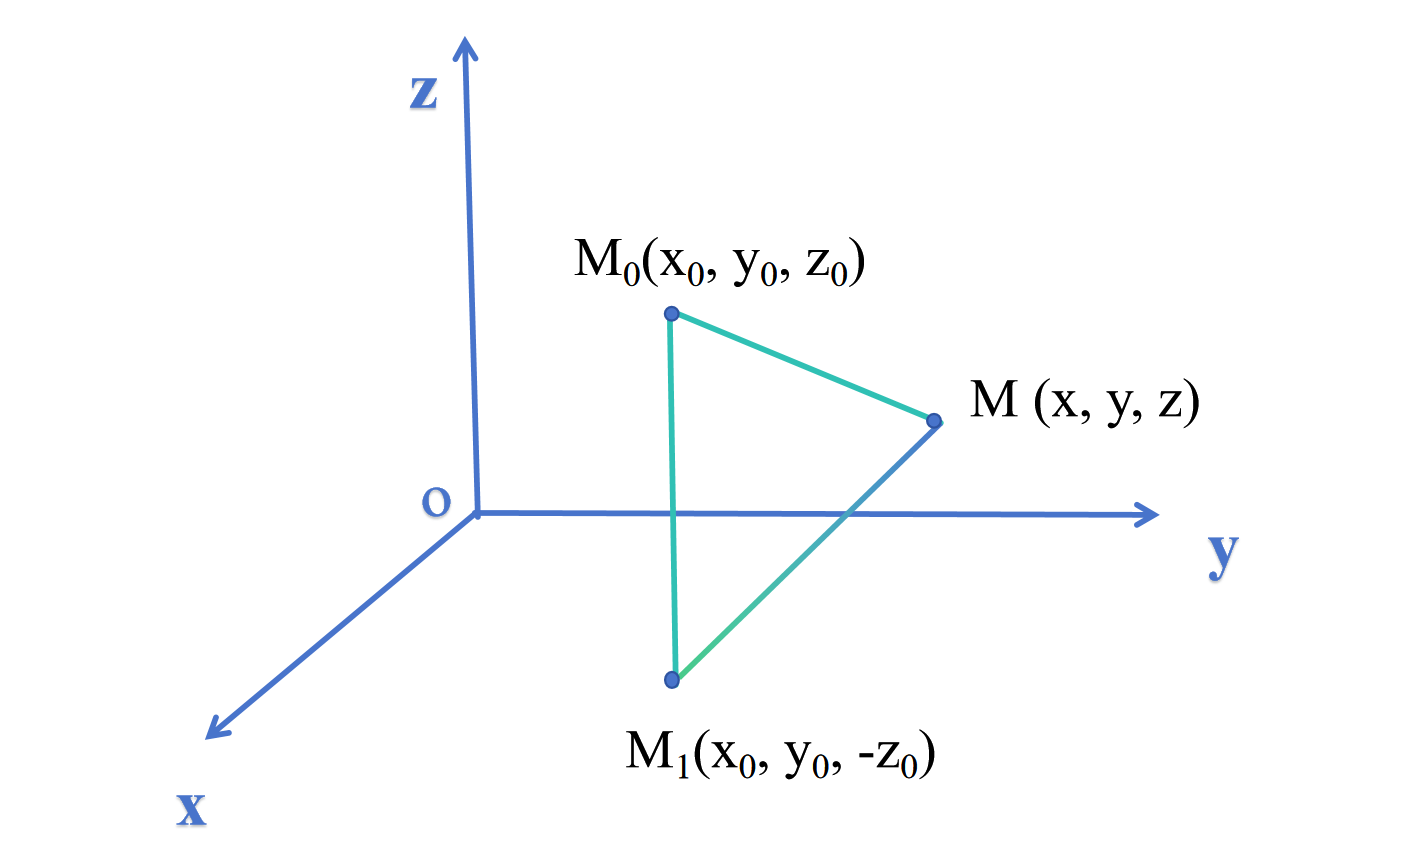
\includegraphics[width=10cm]{pic1.png}
	%\caption{售猪问题的净收益$f(x)$关于售猪时间$x$的曲线图}
\end{figure}
\question{
证明如下方程初边值问题
$$
\left\{\begin{array}{l}
u_{t}=u_{x x}+u, \quad 0<x<l, t>0, \\
u(0, t)=\mu_{1}(t), u(l, t)=\mu_{2}(t), t>0, \\
u(x, 0)=\varphi(x),
\end{array}\right.
$$
解的唯一性与对初值的连续依赖性.
}
\begin{solution}
    作变换 $ v(x, t)=e^{-t} \cdot u(x, t) $ 则 $ v(x, t) $ 满足
$$
\left\{\begin{array}{l}
v_{t}=v_{x x} \quad 0 < x < l, t>0 \\
v(x, 0)=\varphi(x) \quad 0 < x < l \\
v(0, t)=e^{-t} \cdot \mu_{1}(t), v(1, t)=e^{-t} \cdot \mu_{2}(t)
\end{array}\right.
$$

不妨设 $ v_{1}(x, t) , v_{2}(x, t) $ 是该问题的两个解记 $ v(x, t)=v_{1}(x, t)-v_{2}(x, t) $ ,那么 $ v(x, t) $ 满足齐次初边值条件的定解问题
$$
\begin{array}{l}
\left\{\begin{array}{l}
v_{t}=v_{x x} \quad 0 < x < l, t>0 \\
v(x, 0)=0 \quad 0 < x < l \\
v(0, t)=v(l, t)=0 . \quad t > 0 .
\end{array}\right. \\
\end{array}
$$
 对任意一点 $\left(x_{0}, t_{0}\right), \quad 0 \leq x_{0} \leq l, t_{0}>0$
记 $Q=\left\{(x, t) \mid 0 \leqslant x \leqslant l,0 \leqslant t \leqslant t_{0}\right\}$ 其抛物边界为 $ \Gamma $
那么 $ v(x, t) $ 在在 $ \overline{Q} $ 上连续,且满足 $ v_{t}=v_{x x}, 0< x < l , 0 < t \leqslant t_{0} $
由极值原理, 对 $ \forall(x, t) \in \overline{Q} $, 成立如下:
$$
0=\min _{\Gamma} v(x, t) \leqslant v(x, t) \leqslant \max _{\overline{Q}} v(x, t)=0
$$

即在区域 $ \overline{Q} 上, v(x, t)=0 $
特别地 $ v\left(x_{0}, t_{0}\right)=0 \Rightarrow v_{1}\left(x_{0}, t_{0}\right)=v_{2}\left(x_{0}, t_{0}\right) $ ,由于 $ \left(x_{0}, t_{0}\right) $ 是任意的
所以 $ v_{1}(x, t)=v_{2}(x, t) \quad 0 < x < l, t>0 $.
故 $ v(x, t) $ 唯一,也即 $ u(x, t) $ 唯一。

下面考虑解对初值的连续依赖性:

设 $v_{i}(x, t) $ ,$i=1,2$ 是下面问题 
$$\left\{\begin{array}{l}v_{t}=v_{x x} \\ v(x, 0)=\varphi_{i}(x) \\ v(0, t)=e^{-t} \mu_{1}^{(i)}(t), v(l, t)=e^{-t} \mu_{2}^{(i)}(t)\end{array}\right. $$
的解,令 $ v(x, t)=v_{1}(x, t)-v_{2}(x, t) $. $ \varphi(x)=\varphi_{1}(x)-\varphi_{2}(x) $.
$$
f(t)=e^{-t}\left(\mu_{1}^{(1)}(t)-\mu_{1}^{(2)}(t)\right) \quad g(t)=e^{-t}\left(\mu_{2}^{(1)}(t)-\mu_{2}^{(2)}(t)\right)
$$

那么由极值原理得 
$$|v(x, t)|< \varepsilon ,|u(x, t)|= \left|v(x, t) \cdot e^{t}\right|<\varepsilon e^{t} $$
即得证.

\end{solution}
\end{questions}


\subsection{补充内容}

1. 偏微分方程只给出初始条件而没有给出边界条件时,通常称为初值问题(Initial Value Problem,简称IVP)。在这种问题中,你需要通过给定的初始条件找到方程的解。

2. 解的存在、唯一性和稳定性通常被称为问题的适定性。这些属性是用来评估偏微分方程问题是否具有良好的解性质的重要因素。存在性指的是是否存在解,唯一性指的是解是否唯一,稳定性指的是解在输入条件的小变化下是否保持稳定。

3. 设 $ M_{0}=M_{0}\left(x_{0}, y_{0}, z_{0}\right) $ 是空间 $ \mathbb{R}^{3} $ 中某一固定点, $ M=M(x, y, z) $ 是 $ \mathbb{R}^{3} $ 中的动点, 定义函数
$$
v=-\frac{1}{4 \pi r_{M M_{0}}}=-\frac{1}{4 \pi \sqrt{\left(x-x_{0}\right)^{2}+\left(y-y_{0}\right)^{2}+\left(z-z_{0}\right)^{2}}}
$$
这里 $ r_{M M_{0}} $ 表示空间 $ M_{0} $ 与 $ M $ 两点之间的距离.

4. 二维齐次热传导方程的一般形式如下:
$$ u_t = a^2(u_{xx} +u_{yy})$$
在这个方程中,$u$ 是温度分布随时间和空间坐标 $(x, y)$ 的函数,$u_{t}$ 表示温度随时间的变化率,$a^2$ 是热传导系数,$u_{xx}$ 和 $u_{yy}$ 分别表示温度在 $x$ 和 $y$ 方向上的二阶空间导数。这方程描述了热传导过程,其中热量以时间 $t$ 为变量在空间中传导。热传导方程通常用来描述热传导过程中温度分布的演化。它可以通过适当的边界条件和初始条件来解决,以确定在给定时间和空间位置的温度分布。

5. $ u_{t}-\left(u_{xx}+u_{yy}\right)=0 $ 是类型为抛物型的偏微分方程。抛物型偏微分方程通常与时间和空间的二阶导数相结合,通常用于描述稳态或伪稳态过程,如热传导和扩散。这种类型的方程通常具有初始条件和边界条件,以唯一确定解的行为。

6. 物理现象初始状态的条件通常称为初始条件,而说明边界约束情况的条件通常称为边界条件。

初始条件是在时间 $t = 0$ 时对系统的状态或参数进行描述,它们提供了问题的初始时刻的信息。在偏微分方程问题中,初始条件通常是关于时间 t 的解函数及其导数的函数值。

边界条件是在空间中指定系统的行为或性质,通常在问题的边界或边界附近提供。它们约束了问题的解在空间域的边界上的行为,确保解在边界处满足特定条件,如固定值、导数值或其他物理条件。

这两种条件通常结合在一起,以唯一确定偏微分方程问题的解。

7. 边界条件 
$$ \left.\left(\frac{\partial u}{\partial n}+\sigma u\right)\right|_{\partial \Omega}=f $$
是第三类边界条件, 其中 $ \partial \Omega $ 为边界.

在这个条件中,$ \frac{\partial u}{\partial n} $ 表示相对于边界法向量的导数,$ \sigma $ 是给定的参数,$ f $ 是已知的函数。第三类边界条件要求解函数 $ u $ 在边界 $ \partial \Omega $ 上满足与沿边界的外法线方向导数的特定的线性组合。

